
\newif\ifslides\slidestrue
%\slidesfalse

\ifslides
    \documentclass[12pt,envcountsect]{beamer}
    \usepackage{amssymb,amsmath,url}
    \usepackage{pgfplots}
    \setlength{\parskip}{1ex}
\else
    \documentclass[10pt,a4paper]{article}
    \usepackage{amsthm,amssymb,amsmath,hyperref,fancyhdr,boxedminipage,graphics,color}
    \usepackage[envcountsect]{beamerarticle}
    \pagestyle{fancyplain}
    \lhead[\fancyplain{}{\thepage}]{\fancyplain{}{}}
    \cfoot{}
    \rhead[\fancyplain{}{}]{\fancyplain{}{\thepage}}
    \setlength{\parskip}{1em}
    \setlength{\parindent}{0em}
    \renewcommand{\baselinestretch}{1.2}
    \setlength{\skip\footins}{16pt}
\fi

\newif\iftitled\titledtrue

\usepackage[latin1]{inputenc}
\usepackage[english]{babel}
\usepackage{pdfpages}
\usetheme{Pittsburgh}
\usefonttheme[stillsansseriftext]{serif}
\usefonttheme{structurebold}

% Choose and set background colour
\definecolor{bgcolour}{RGB}{255,255,245}
\setbeamercolor{background canvas}{bg=bgcolour}
\setbeamercolor{example text}{fg=black}

% Set-up a custom header strip
\definecolor{headercolour}{RGB}{255,255,255}
\definecolor{bordercolour}{RGB}{255,0,68}
\definecolor{palegrey}{RGB}{180,180,180}
\definecolor{darkergrey}{RGB}{100,100,100}
\setbeamercolor{headerstrip}{fg=black,bg=white}
\setbeamercolor{border}{fg=black,bg=bordercolour}
\setbeamercolor{top strip}{fg=black,bg=palegrey}
\setbeamercolor{bottom strip}{fg=black,bg=darkergrey}
\setbeamercolor{structure}{fg=black}

%sets top border strip
\setbeamertemplate{headline}
{
  \begin{beamercolorbox}[wd=\paperwidth,ht=0ex,dp=1.2ex]{headerstrip}%
  \end{beamercolorbox}%
  \begin{beamercolorbox}[wd=\paperwidth,ht=0ex,dp=0.2ex]{top strip}%
  \end{beamercolorbox}
  \begin{beamercolorbox}[wd=\paperwidth,ht=0ex,dp=0.2ex]{border}%
  \end{beamercolorbox}
  \begin{beamercolorbox}[wd=\paperwidth,ht=0ex,dp=0.3ex]{bottom strip}%
  \end{beamercolorbox}
  \begin{beamercolorbox}[wd=\paperwidth,ht=0ex,dp=4ex]{background canvas}%
  \end{beamercolorbox}
}

%gets rid of bottom navigation bars
\setbeamertemplate{footline}
{
  \begin{beamercolorbox}[wd=\paperwidth,ht=0ex,dp=0.2ex]{top strip}%
  \end{beamercolorbox}
  \begin{beamercolorbox}[wd=\paperwidth,ht=0ex,dp=0.2ex]{border}%
  \end{beamercolorbox}
  \begin{beamercolorbox}[wd=\paperwidth,ht=0ex,dp=0.3ex]{bottom strip}%
  \end{beamercolorbox}
  \begin{beamercolorbox}[wd=\paperwidth,ht=0ex,dp=1.2ex]{headerstrip}%
  \end{beamercolorbox}
}

%gets rid of navigation symbols
\setbeamertemplate{navigation symbols}{}

%removes italics from theorems, problems etc
\setbeamertemplate{theorems}[ams style]

%makes quotes italic in beamer article mode
\mode<article>{
  \renewenvironment{quote}{\actionenv\begin{itshape}\originalquote}{\endoriginalquote\end{itshape}\endactionenv}
}

%makes line breaks work in article mode
\makeatletter
\let\beamer@@breaker\beamer@origbreak
\let\beamer@@breakercenter\beamer@origbreakcenter
\makeatother

%makes enumerate lists nice and plain
\setbeamertemplate{enumerate item}{(\roman{enumi})}

%makes frametitles etc on the left
\mode<presentation>{\setbeamertemplate{frametitle}[default][left]}


%sets up how to introduce new sections
\AtBeginSection
[
\begin{frame}
  \usebeamerfont{section title}{\bf ~\insertsection}
  \vspace{5cm}~
\end{frame}
\addtocounter{section}{-1}
]
{
\begin{frame}
  \usebeamerfont{section title}{\bf ~\insertsection}
  \vspace{5cm}~
\end{frame}
}

\AtBeginSubsection
[
\begin{frame}
  \usebeamerfont{section title}{\bf ~\insertsubsection}
    \vspace{5cm}~
\end{frame}
]
{
\begin{frame}
  \usebeamerfont{section title}{\bf ~\insertsubsection}
    \vspace{5cm}~
\end{frame}
}

\AtBeginSubsubsection
[
\begin{frame}
  \usebeamerfont{section title}{\sc ~\insertsubsubsection}
    \vspace{5cm}~
\end{frame}
]
{
\begin{frame}
  \usebeamerfont{section title}{\sc ~\insertsubsubsection}
    \vspace{5cm}~
\end{frame}
}

\newcommand{\ipause}{\pause[\thebeamerpauses]}
\newcommand{\iipause}{\pause[\thebeamerpauses+1]}

\newcommand{\R}{{\mathbb R}}
\newcommand{\N}{{\mathbb N}}
\newcommand{\Q}{{\mathbb Q}}
\newcommand{\C}{{\mathbb C}}
\newcommand{\Z}{{\mathbb Z}}
\newcommand{\uda}{\updownarrow}
\newcommand{\ov}{\overline}
\newcommand{\send}{\mathop{\rm send}\nolimits}
\newcommand{\rot}{\mathop{\rm rot}\nolimits}
\newcommand{\refl}{\mathop{\rm ref}\nolimits}
\newcommand{\sgn}{\mathop{\rm sgn}\nolimits}
\newcommand{\stab}{\mathop{\rm stab}\nolimits}
\newcommand{\odd}{\mathop{\rm odd}\nolimits}
\newcommand{\even}{\mathop{\rm even}\nolimits}
\newcommand{\swop}{\mathop{\rm swop}\nolimits}
\newcommand{\cl}{\mathop{\rm cl}\nolimits}
\newcommand{\anticl}{\mathop{\rm anticl}\nolimits}
\newcommand{\orb}{\mathop{\rm orb}\nolimits}
\newcommand{\id}{\mathop{\rm id}\nolimits}
\newcommand{\fix}{\mathop{\rm fix}\nolimits}
\newcommand{\la}{\langle}
\newcommand{\ra}{\rangle}
\newcommand{\st}{{\mbox{st}}}

\newcommand{\q}{{\bf Question. }}
\newcommand{\leadingword}[1]{\textbf{#1}}

\theoremstyle{plain}
\newtheorem{thm}[theorem]{Theorem}
\newtheorem{prop}[theorem]{Proposition}
\newtheorem{cor}[theorem]{Corollary}

\theoremstyle{definition}
\newtheorem{defn}[theorem]{Definition}
\newtheorem{defns}[theorem]{Definitions}
\newtheorem{rmk}[theorem]{Remark}
\newtheorem{rmks}[theorem]{Remarks}
\newtheorem*{eg}{Example}
\newtheorem*{egs}{Examples}
\newtheorem*{Note}{Note}
\newtheorem*{notes}{Notes}
\newtheorem{algor}[theorem]{Algorithm}
\newtheorem{gloss}[theorem]{Glossary}

%environments for indenting text
\newenvironment{intext}{\begin{center}\begin{minipage}{10cm}} {\end{minipage}\end{center}}
\newenvironment{ittext}{\begin{intext}\begin{center}\em} {\end{center}\end{intext}}
\newenvironment{boxtext}{\begin{center}\begin{boxedminipage}{10cm}\begin{center} \bf } {\end{center}\end{boxedminipage}\end{center}\smallskip}

% --Notes for students (with blanks)---------
\newenvironment{btext}{\begin{color}{white}} {\end{color}}
\newenvironment{bmfpic}[6]{\begin{color}{white}\begin{mfpic}[#1][#2]{#3}{#4}{#5}{#6}\drawcolor{white}\fillcolor{white}\tlabelcolor{white}\hatchcolor{white}\headcolor{white}\pointcolor{white}} {\end{mfpic}\end{color}}
\newcommand{\shd}{}
%------------------------

%% --Complete notes------
%\newenvironment{btext}{}{}
%\newenvironment{bmfpic}[6]{\begin{mfpic}[#1][#2]{#3}{#4}{#5}{#6}} {\end{mfpic}}
%\newcommand{\shd}{\shade[1]}
%%------------------------





\newenvironment{activity}{\vspace{1ex}\noindent\textbf{Activity.}~}{}
\newenvironment{announcement}{\begin{center}\bf\large}{\end{center}}

\begin{document}

\title{A new approach to our engineering teaching\\
\begin{small}(aka engaging large groups through blended learning)\end{small}}
\author{Sam Marsh}
\date{January 2014}

\mode<article>{
    \iftitled\maketitle\fi
}

\mode<presentation>{
    \iftitled
        \begin{frame}
        \titlepage
        \end{frame}
    \fi
}

\section{Background}

\begin{frame}
Most engineering students learn mathematics on modules taught by us. \pause Traditionally, we've used the standard format: two lectures per week \pause ($240$ students or more), \pause and a problem class once a week \pause ($\sim 40$ students, sometimes more).\pause

Attendance at problem classes has tended to taper off as the semester progresses.
\end{frame}


\begin{frame}
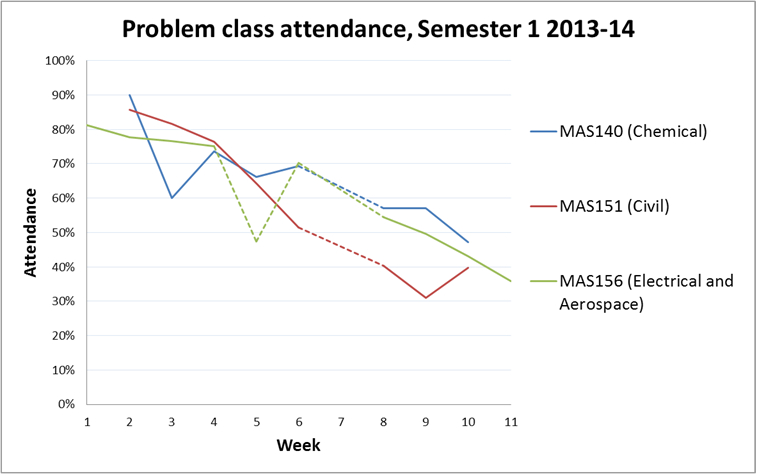
\includegraphics[width=1\textwidth]{attendance_chart_1.png}\pause

{\scriptsize
\begin{itemize}
\item Week 7 was a reading week; \pause MAS156 was affected by strike action in Week 5.\pause
\item MAS140 and MAS151 had class tests in Week 11 (data omitted).
\end{itemize}
}
\end{frame}

\begin{frame}
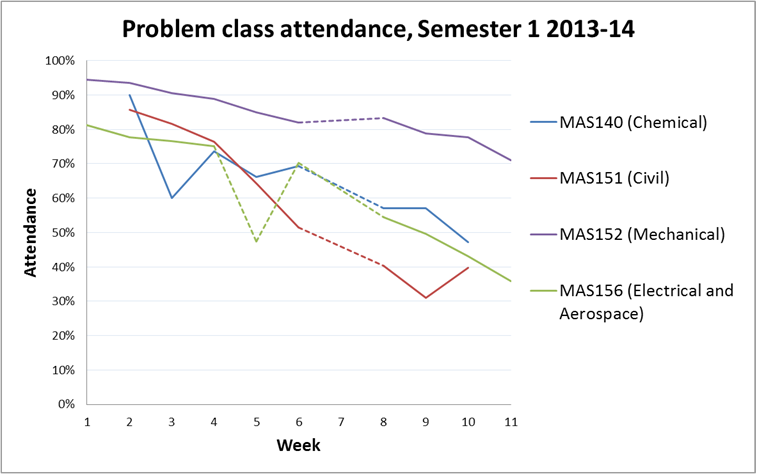
\includegraphics[width=1\textwidth]{attendance_chart_2.png}

{\scriptsize
\begin{itemize}
\item MAS152 is a new format pilot module.\pause
\item Feedback from the staff-student forum has been very positive.
\end{itemize}
}
\end{frame}

\section{About the new format}

\begin{frame}
Mechanical engineering agreed to a pilot of a new format for their Level 1 students. \pause This format uses a blended approach, with \pause
\begin{itemize}
\item short (10--15 minute) video lectures replacing face-to-face lectures;\pause
\item short (3 question) online tests following each video;\pause
\item restructured, more interactive problem classes \pause (and double the number);\pause
\item all backed up with course notes and exercise sheets as before, \pause a MOLE discussion board \pause and three full-class lectures each Semester.\pause
\end{itemize}
(This format was devised by Nick Gurski, based on videos made by Simon Willerton and Eugenia Cheng, and with input from Stephen Beck in Mechanical Engineering.)
\end{frame}

\begin{frame}
The pattern for the week is as follows.\pause
\begin{itemize}
\item Three videos are released on Tuesday; \pause students watch them before their problem class on Thursday/Friday.\pause
\item Three videos are released on Friday; \pause students watch them before their problem class on Monday/Tuesday.
\end{itemize}
\end{frame}

\begin{frame}
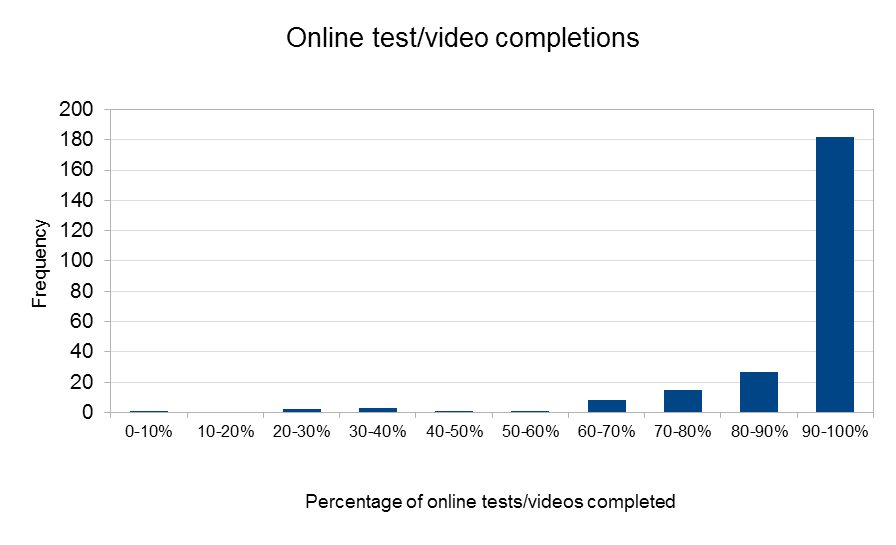
\includegraphics[width=1\textwidth]{video_completions.png}

{\scriptsize
\begin{itemize}[<+->]
\item In Semester 1, $75\%$ of students completed $90\%$ or more of the videos on time.
\item $98$ of the $240$ students completed all of the videos on time.
\end{itemize}
}
\end{frame}

\subsection{The videos}

\begin{frame}
The videos are short `chalk and talk' lectures filmed specially for purpose \pause (not recordings of live lectures). \pause We used minimal equipment \pause (video camera, \pause two umbrella lights, \pause a lapel mic) \pause but the results are good enough. \pause Most important is the content and delivery.\pause

We've managed to find a room in SoMaS which will be a semi-permanent studio for any staff who would like to make videos. \pause We'll make announcements when it's ready to be used.
\end{frame}

\subsection{The delivery system}

\begin{frame}
The videos are delivered through the Assessment in Mathematics (AiM) online testing system developed by Neil Strickland and others. \pause This allows us to follow each video with online tests which can test mathematics in a sophisticated way. \pause My understanding is that MOLE can do most of what we needed.\pause

Details about AiM can be found at \url{http://aim.shef.ac.uk/AiM/doc/}, or ask Neil or Simon or Eugenia or me or\ldots
\end{frame}



\subsection{The problem classes}

\begin{frame}
The problem classes are the focus of the module. \pause Each class of 40 students is run by one tutor. \pause The tutor is given a sheet specifying material to recap (5-minute review), \pause an example or two to do with class input, \pause and some interesting exercises for the students to work on. \pause

Students are encouraged to work in a groups of 4 on the problems, \pause meeting people in the process. \pause Tutors report their students engaging well with the material and using the class productively, \pause which hasn't always been the case in the past.
\end{frame}

\section{Speculation}

\begin{frame}
Everything points to this new format working well. \pause Here are some thoughts on why that might be the case.\pause
\begin{itemize}
\item Attendance: \pause students only have to attend problem classes, \pause so are more likely to do so. \pause We think they also find the classes more useful than before.\pause
\item Students have to watch the videos to gain credit for the tests, \pause so are more likely to do so than attend lectures.\pause
\item Students can choose when to watch videos, \pause and re-watch them as necessary.\pause
\item Problem classes recap the material briefly, reinforcing learning.\pause
\item The students experience the course as if they are in a group of size 40 rather than 240 \pause and get to know their tutor well.
\end{itemize}
\end{frame}

\section{Course materials}

\begin{frame}
You can view the materials for the module on the course webpage, \url{http://sam-marsh.staff.shef.ac.uk/mas152}.

You can try out the video system using the link below.

\url{http://aim.shef.ac.uk/AiM/Alice?SubjectName=Test}

username:\texttt{engineering}, password:\texttt{letmein}
\end{frame}

\end{document} 